\documentclass{article}
\usepackage[utf8]{inputenc}
\usepackage{array,multirow,graphicx}
\usepackage{amsmath,amssymb,latexsym}
\usepackage{mathabx}
\usepackage{parskip}
\usepackage{listings}
\usepackage[section]{placeins}
\usepackage{hyperref}
\usepackage[english]{babel}
\usepackage{biblatex}
\renewcommand{\sfdefault}{ptm}
\graphicspath{ {/} }

\title{Report.7.View}
\author{Linh Duong}
\date{November 2017}

\begin{document}

\maketitle

\section{Who have the same name as the managers of the “Finance” department?}
\begin{lstlisting}[language=sql]
create view ManagerLastName as 
select last_name from employees 
join dept_manager on employees.emp_no = dept_manager.emp_no
join departments on departments.dept_no=dept_manager.dept_no 
and dept_name='Finance';

select distinct employees.emp_no,concat(first_name,' ',last_name) 
as fullname
from employees join dept_emp on employees.emp_no=dept_emp.emp_no 
	join departments on departments.dept_no=dept_emp.dept_no
where last_name in (select * from ManagerLastName);
\end{lstlisting}
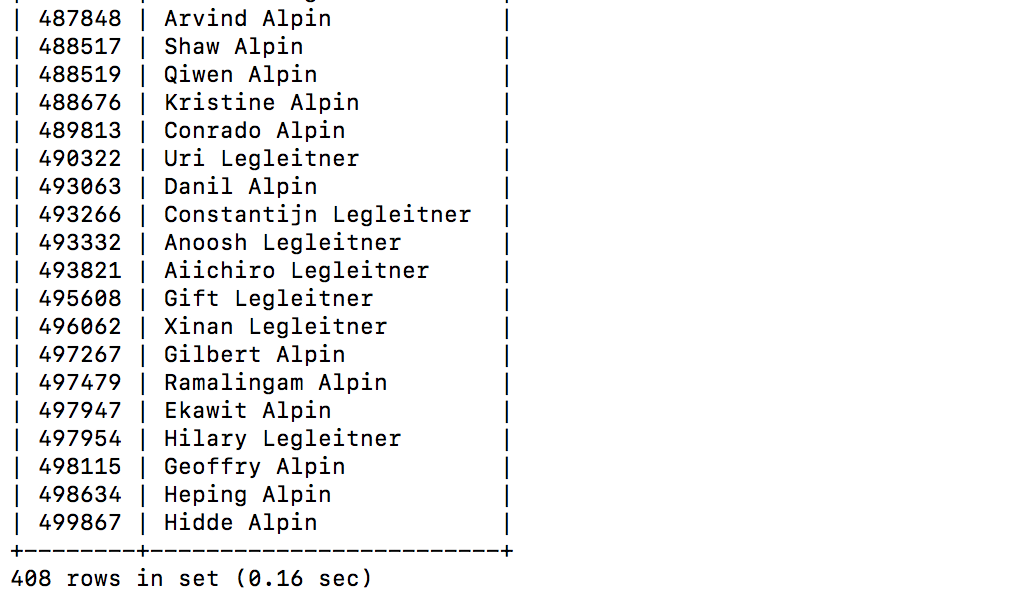
\includegraphics[width=\linewidth]{1.png}

\section{Who in the “Production” department were hired after the promotion of the last manager in that department?}
\begin{lstlisting}[language=sql]
create view ManagerPromotion as
select from_date from dept_manager 
where dept_no = (select dept_no 
	from departments where dept_name='Production') 
order by from_date desc limit 0,1;

select employees.emp_no,concat(first_name,' ',last_name) 
as fullname
from employees 
join dept_emp on employees.emp_no=dept_emp.emp_no 
join departments on departments.dept_no=dept_emp.dept_no 
and dept_name='Production'
where from_date > ( select * from ManagerPromotion);

\end{lstlisting}
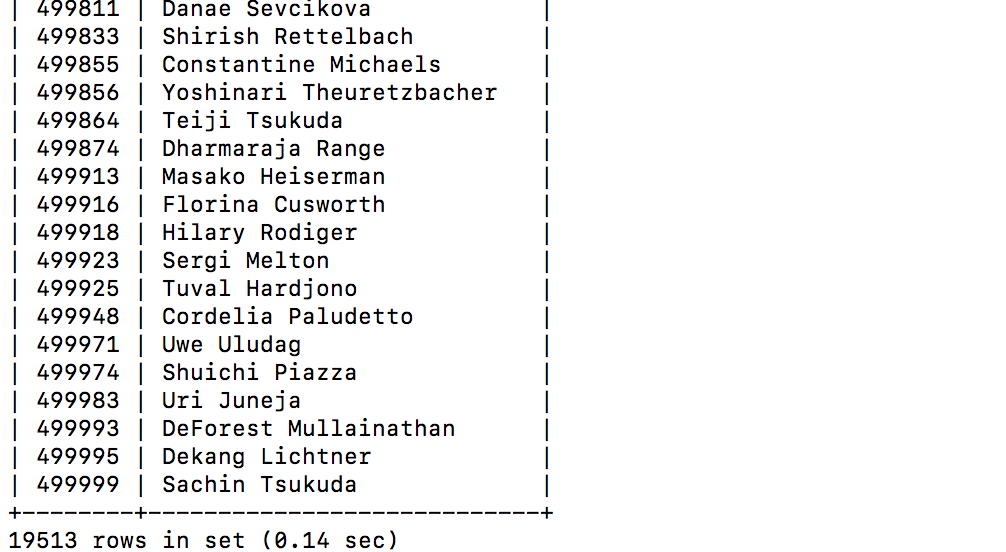
\includegraphics[width=\linewidth]{2.png}

\section{Find the average salary of each department, from highest to lowest.}
\begin{lstlisting}[language=sql]
create view AvgSalary as
select dept_emp.dept_no, dept_name, avg(salary) as average 
from salaries 
join employees on employees.emp_no=salaries.emp_no 
join dept_emp on dept_emp.emp_no = employees.emp_no
join departments on dept_emp.dept_no = departments.dept_no
group by dept_emp.dept_no ;

select dept_name, average from AvgSalary
order by average desc;
\end{lstlisting}
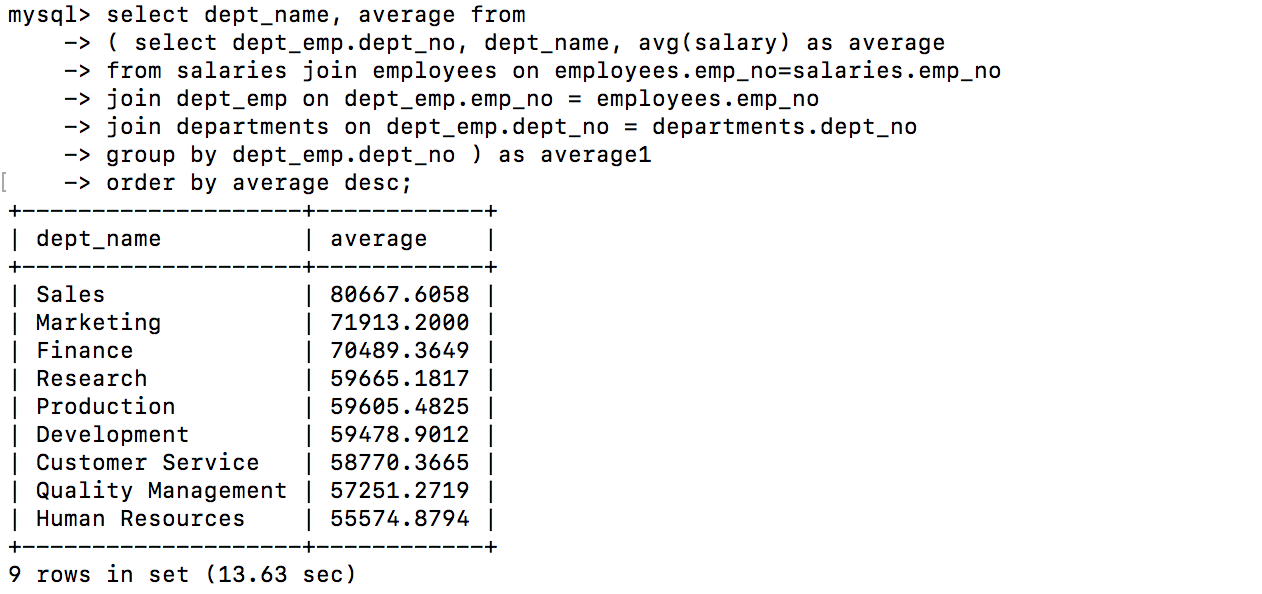
\includegraphics[width=\linewidth]{3.png}

\section{Find the average salary for each type of Engineer, from highest to lowest.}
\begin{lstlisting}[language=sql]
create view AvgSal as
select emp_no,avg(salary) as avgsalary
from salaries group by emp_no;

select title, avg(avgsalary) as averagesalary
from AvgSal join titles on AvgSal.emp_no=titles.emp_no 
and title like '%Engineer%'
group by title
order by averagesalary desc;
\end{lstlisting}
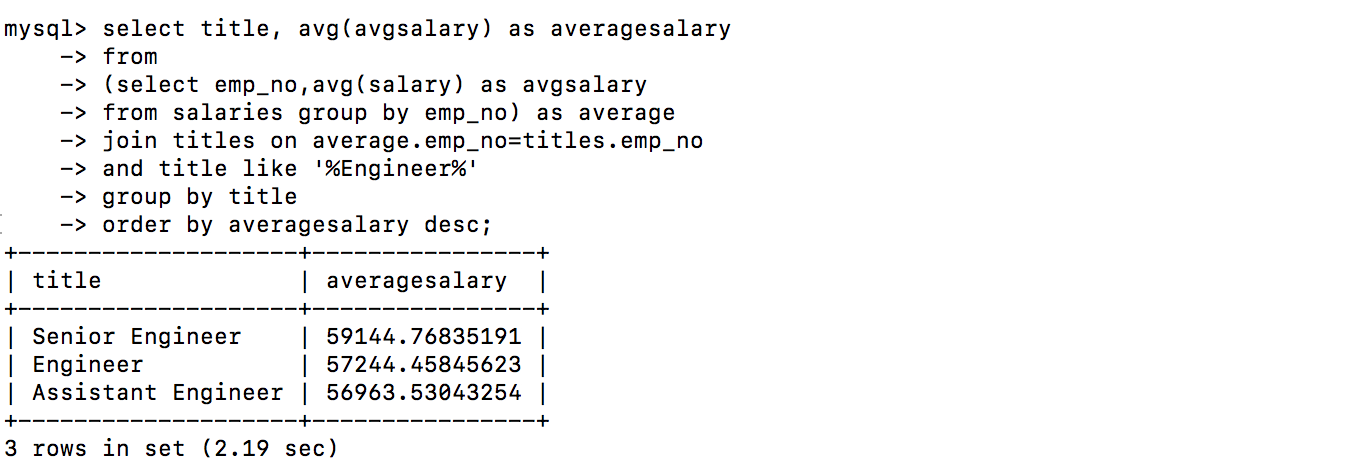
\includegraphics[width=\linewidth]{4.png}


\end{document}